\setcounter{chapter}{-1}
\setchapterabstract{This chapter explores the legal framework on market dominance abuse under Article 102 TFEU, defining "dominance" as significant market power enabling an undertaking to operate independently in a market without effective competition constraints. However, dominance itself is lawful; it is its abuse that Article 102 prohibits. Abusive practices, either exploitative or exclusionary, harm competition by distorting market conditions or limiting consumer choice and innovation. Examples include imposing unfair trading conditions or limiting production. The Digital Markets Act (DMA) adds specific rules for digital gatekeepers, enhancing fairness in the market. Enforcement requires a structural element (dominance) and a behavioural element (abusive conduct), with defences like efficiency gains considered only if they do not disproportionately restrict competition.}
\chapter{Concepts of dominance and its abuse}
\vspace{-1.5cm}

\setcounter{chapter}{10}
{\chaptoc\noindent\begin{minipage}[inner sep=0,outer sep=0]{0.9\linewidth}\section{Article 102 TFEU}\end{minipage}}

    \subsubsection{Article 102(1)}

        \begin{quote}
            “Any abuse by one or more undertakings of a dominant position within the internal market or in a substantial part of it shall be prohibited […] in so far as it may affect trade between Member States […]
        \end{quote}

        \begin{enumerate}
            \item Significant market power (dominant position) 
            \item Unilateral conduct (no need for an agreement) 
            \item Conduct that abuses market power 
            \item Capable of at least potential (anticompetitive) effects
        \end{enumerate}

    \subsubsection{Article 102(2)}

        \begin{quote}
            Such abuse may, in particular, consist in:
            \begin{enumerate}[label=\alph*.]
                \item directly or indirectly imposing unfair purchase or selling prices or other unfair trading conditions; 
                \item limiting production, markets or technical development to the prejudice of consumers;
                \item applying dissimilar conditions to equivalent transactions with other trading parties, thereby placing them at a competitive disadvantage;
                \item making the conclusion of contracts subject to acceptance by the other parties of supplementary obligations which, by their nature or according to commercial usage, have no connection with the subject of such contracts.”
            \end{enumerate}
        \end{quote}

    \subsection{Enforcement policy}

        Given that in a monopolistic equilibrium consumer and total surplus are lower than in a competitive equilibrium, should becoming dominant be prohibited?

\noindent
        No, we need to incentivize competition to gain sales (and potentially win the market) as it delivers innovation, efficiencies and lower prices.


        We want everyone to keep improving and doing their best to succeed, with the prospect of enjoying the (even monopolistic) fruits of their efforts. Although not without limitations. Limiting firms’ unilateral conduct before they reach dominance may have a chilling effect on competition and lead to an oligopolistic equilibrium

\section{Digital Markets Act}

    To address perceived limitations of competition law in digital markets, in terms of enforcement taking too long and remedies being ineffective, the EU adopted a new regulation – the \textbf{Digital Markets Act (DMA)}. Designated companies have to comply by March 2024.
    
    The DMA creates a new set of rules, mostly inferred from past and ongoing EC investigations, to foster fairness and contestability. The DMA applies to a small number of firms called “gatekeepers,” identified based on:
    \begin{enumerate}[label=(\roman*)]
        \item market capitalization or annual turnover,
        \item provision of one of the listed core platform services (digital services connecting business users to end users), and
        \item reaching certain user thresholds.
    \end{enumerate}
    
    By October 2024, 7 gatekeepers were designated (excluding Booking.com – X was not designated).
    
    The EC started non-compliance investigations against the following:
    
    \begin{itemize}
        \item \textbf{Google:}
        \begin{itemize}
            \item Anti-steering practices, limiting developers’ ability to inform their customers of alternative, cheaper purchasing possibilities in Google Play.
            \item Self-preferencing on Google Search, favouring services like Google Shopping, Google Flights, and Google Hotels.
        \end{itemize}
        \item \textbf{Apple:}
        \begin{itemize}
            \item Anti-steering practices in the App Store $\rightarrow$ \textit{Preliminary finding of a breach}.
            \item Ineffective choice screen in Safari for selecting a different default browser or search engine $\rightarrow$ \textit{Changes made}.
            \item New contractual requirements for third-party app developers regarding alternative distribution and app stores to access iOS.
        \end{itemize}
        \item \textbf{Meta:} The “pay or consent model” $\rightarrow$ \textit{Preliminary finding of a breach}.
    \end{itemize}
    
    The EC has also opened a specification proceeding regarding Apple’s interoperability obligations concerning iOS.

        \subsubsection{With great (market) power comes special responsibility}

            Article 102 does not prohibit dominance. It prohibits its abuse.
            Obtaining, enjoying, and even strengthening a dominant position
            is not prohibited \textit{per se}.
            
            However, certain unilateral conducts are prohibited if the firm
            adopting them is in a position of market power (a “dominant
            position”).
            
            A violation of Article 102 is thus composed of (you need both!):
            \begin{enumerate}
                \item a structural element (dominance)
                \item a behavioural element (abusive conduct)
            \end{enumerate}

    \subsection{Purpose of Article 102}

    \begin{enumerate}[label=\roman*.]
        \item In protecting an effective competitive process, the EC will intervene only if the conduct is hampering competition from as-efficient competitors.
        \item “The emphasis of the Commission's enforcement activity in relation to exclusionary conduct is on safeguarding the competitive process […] and ensuring that undertakings which hold a dominant position do not exclude their competitors by other means than competing on the merits […]. This may well mean that competitors who deliver less to consumers in terms of price, choice, quality, and innovation will leave the market.”
        \item “The Commission will normally only intervene where the conduct […] is capable of hampering competition from competitors which are considered to be as efficient as the dominant undertaking.”
    \end{enumerate}

\section{The structural element: Dominant Position}

    The unilateral behaviour of an undertaking is subject to scrutiny only where that undertaking is dominant.\sn{\Note{Market definition is key to the dominance assessment:
            \begin{itemize}
                \item Product Market
                \item Geographic Market
            \end{itemize}}}
    Neither the Treaty nor regulations provide a definition of dominance, so we must turn to the case law:
        \begin{quote}
            “The dominant position […] relates to a position of economic strength […] which enables [the undertaking] to prevent effective competition being maintained on the relevant market by affording it the power to behave to an appreciable extent independently of its competitors, customers and ultimately of its consumers.”
        \end{quote}

        \subsubsection{How can we determine if a firm is dominant?}
    
            \begin{itemize}
                \item It enjoys a substantial level of market power.
                \item To determine market power, we look at the degree of competitive constraint exerted by:
                \begin{enumerate}
                    \item \textbf{actual} competitors,
                    \item \textbf{potential} competitors, and
                    \item \textbf{customers} (countervailing buyer power).
                \end{enumerate}
                \item When these competitive constraints are ineffective, the undertaking enjoys substantial market power as it can make business decisions disregarding competitors’ and customers’ reactions.\sn{\Note{\(\Rightarrow\) The undertaking can profitably increase or fix prices substantially above the competitive level and persist in doing so without erosion of its market position or expansion by potential or actual rivals.}}
            \end{itemize}

    \subsection{1st Competitive Constraint: Actual Competitors}

        Players currently competing with the undertaking whose dominance is to be determined – i.e., companies offering substitutable products. Market shares provide a useful indication of the market structure and of the relative importance of players active in it. In zero-price markets, the number of users, transactions, and intensity of usage may provide better indications to determine market power.
        
        However, market shares may not be indicative of market power. You need to account for market dynamics:
        \begin{enumerate}[label=\roman*.]
            \item trend of development of market shares\sn{stable position over time or volatile market},
            \item fast-growing markets with short innovation cycles,
            \item lump orders,
            \item bidding market,
            \item product differentiation\sn{closely competing products, similar technology, same customers…},
            \item players’ relative position\sn{similar shares or material gap, fragmented or concentrated}, and
            \item firm’s profitability.
        \end{enumerate}

        \subsubsection{Market shares and the Akzo presumption}

            \begin{quote}
                “Although the importance of the market shares may vary from one market to another […] very large shares are in themselves, and save in exceptional circumstances, evidence of the existence of a dominant position. An undertaking which has a very large market share and holds it for some time […] is by virtue of that share in a position of strength.” (CJEU, 85/76, Hoffmann-La Roche)
            \end{quote}
            \begin{quote}
                “That is the situation where there is a market share of 50\%.” (CJEU, C-62/86, Akzo)
            \end{quote}

            A market share of 50\%+ in the relevant market\sn{\Note{but only in the relevant market — first, you must define it!}} leads to a (rebuttable) presumption of dominance (the \textbf{Akzo presumption}).
            It is for the firm to demonstrate that due to market dynamics it does not have market power

        \subsubsection{Market shares – Commission’s guidance for market shares below 50\%}

            \begin{enumerate}[label=\roman*.]
                \item \textbf{No safe harbour}. A market share of ~40-45\% was sufficient, together with other factors, to find dominance. However, even below 40\%, competitors may not be in a position to be effective constraints\sn{e.g., capacity limitations}, and the firm may be in a dominant position.
                \item If the market share is below 10\%, dominance is very unlikely (requires exceptional circumstances).
                \item The higher the market share, and the longer the period over which it is held, the more likely it is an indication of dominance.
                \item The Commission will examine all factors that may constrain the behaviour of the allegedly dominant firm to determine if they are sufficient.
            \end{enumerate}

    \subsection{2nd Competitive Constraint: Potential Competitors}

        Credible threat of:
            \begin{itemize}
                \item expansion by actual competitors,
                \item entry by potential competitors.
            \end{itemize}
        
        Market shares do not show constraint from firms not yet in the market but capable of entering, or from firms already in the market and capable of expanding in case of a price increase (e.g., if the high market share is the result of pricing at or below cost, that is unlikely to signal market power if barriers to entry are low).

        \Remark{Significance of constraint from potential competitors is determined by the barriers to entry and expansion}

        \subsubsection{Entry Barriers}

            \begin{enumerate}
                \item Legal barriers
                \begin{enumerate}[label=\alph*.]
                    \item ownership of intellectual property rights (IPRs),
                    \item licensing / authorization requirements and planning regulation,
                    \item tariff and non-tariff barriers,
                    \item statutory monopolies.
                \end{enumerate}
                
                \item Economic barriers (difficult, expensive, time-consuming to overcome)
                \begin{enumerate}[label=\alph*.]
                    \item control of an essential facility,
                    \item economies of scale and scope,
                    \item broad portfolio,
                    \item vertical integration,
                    \item exclusive access to critical inputs (e.g., raw materials) or customers,
                    \item network effects,
                    \item switching costs / lock-in effects,
                    \item highly developed / established sales and distribution network,
                    \item brand image and reputation,
                    \item customer inertia,
                    \item data-driven advantages,
                    \item first-mover advantages.
                \end{enumerate}
            \end{enumerate}

\newpage
    \subsection{3rd Competitive Constraint: Customers}

        The bargaining strength of customers may counterbalance the market power of the allegedly dominant firm. Can customers make a price increase unprofitable by switching to rival products? (e.g., supermarket chains on one side and suppliers of food/drinks on the other).
        
        \begin{itemize}
            \item Countervailing buyer power can be a significant constraint but only if a (commercially significant amount of) buyer(s) can, for all or most of their purchases:
            \begin{itemize}
                \item (easily and inexpensively) switch to competing suppliers,
                \item integrate vertically (self-supply), or
                \item sponsor the expansion or entry of a new rival.
            \end{itemize}
            \item Buyer power is not an effective constraint if only a limited segment of customers (e.g., few large and sophisticated buyers in a fragmented industry) is shielded from the supplier’s market power or can discipline the supplier in case of a price increase.
        \end{itemize}

    \Example{
    \textbf{Mock Exam | }Coca Cola has X\% market share … of what market?
    \begin{itemize}
        \item Product market
        \begin{itemize}
            \item Colas?
            \item Carbonated beverages?
            \item Sweet beverages?
            \item Non-alcoholic drinks (incl./excl. water)?
            \item Drinks?
        \end{itemize}
        \item Geographic market
        \begin{itemize}
            \item National?
            \item EEA-wide?
            \item Global?
        \end{itemize}
        \item Market power?
        \begin{itemize}
            \item Akzo presumption
            \item Constraints: actual, potential (and barriers), buyers…
        \end{itemize}
    \end{itemize}
    }

\newpage
    \subsection{The behavioural element: the abuse}

        \begin{itemize}
            \item No general and all-encompassing definition or exhaustive list.
            \item Court of Justice of the European Union explained:
            \begin{itemize}
                \item Concept of abuse is objective.
                \item Consists in methods different from those which condition normal competition in products or services.
                \item Abuse must be able to influence (weaken) the structure of the market where, as a result of the presence of the dominant undertaking, competition is already weak.
                \item Has the (actual or potential) effect to hinder the maintenance of the (limited) degree of competition existing or its growth.
                \item To the detriment of consumers.
            \end{itemize}
        \end{itemize}

\section{Competition on the merits}

    Abuse is what deviates from “normal” competition.  
    Normal competition is competition on the ‘merits’ or on ‘performance’.
    
    \begin{itemize}
        \item “Article 102 prohibits […] eliminating a competitor and thereby strengthening [a dominant] position by using methods other than [...] competition on the merits.”
        \item “Competition on the merits may, by definition, lead to the departure from the market or the marginalization of competitors that are less efficient and so less attractive to consumers [on] price, choice, quality or innovation” [these are examples of “merits” / “performance”].
    \end{itemize}
    
    It is thus competition on the merits and not an abuse to eliminate less-efficient competitors and strengthen a dominant position by offering lower prices, better quality, wider choice, and innovative goods and services.
    
    There are a number of economic tests which can aid in the identification of competition on the merits. Each has its drawbacks, but they can be useful as analytical tools:
    
    \begin{itemize}
        \item \textbf{“As-efficient competitor” (AEC) test:} Conducts may be abusive if capable of excluding a competitor having the same characteristics (e.g., costs) as the dominant firm. That is, could (would it be economically possible / rational for) an AEC replicate the dominant undertaking’s conduct, without dominance? The AEC test is not necessary, but when carried out, it must be taken into account.
        \item \textbf{Profit sacrifice/no economic sense test:} Conducts may be abusive if rationality rests only on the restriction of competition. For example, payments to postpone or cancel the launch of competing products, or dismantling an infrastructure used by a competitor.
    \end{itemize}

    \subsection{The role of effects}

        No need to demonstrate concrete anticompetitive effects.  
        It is sufficient, but at the same time necessary, to show that the practice is “liable to,” “capable of,” or “has the tendency to” restrict competition.  

        \Remark{It does not need to be the sole cause. It is sufficient if it increases the likelihood of exclusionary effects materializing; \textbf{but actual effects are considered} in most cases.}
        
        Even in cases where effects may be presumed due to the nature of the conduct, defendants’ evidence on the lack of restrictive impact must be taken into account to determine whether the conduct is capable of foreclosure, considering:
        
        \begin{enumerate}[label=\roman*.]
            \item market power,
            \item share of the market covered by the contested practice,
            \item characteristics of the conduct (targeting important customers or input suppliers?),
            \item duration and frequency of the conduct,
            \item intent (plan/strategy to exclude), and
            \item actual market developments (increase/decline in shares, exits, failed entry).
        \end{enumerate}

        No \textit{de minimis} threshold to determine if a conduct is abusive.  
        Any actual or potential anticompetitive effect of a conduct that departs from competition on the merits will further weaken competition and be captured.
        
        Once (actual or potential) effects are established, there is no need to prove that it is of a serious or appreciable nature.

    \subsection{The role of intent}

        As the notion of abuse is ‘objective’, the characterization of a conduct as abusive does not imply or require fault or the subjective intention to exclude competitors or cause harm.
    
        However, an anti-competitive intention is taken into account to conclude that a conduct is abusive.
        
        The Court took the position that:  
        \begin{quote}
            “establishing the anti-competitive object and the anti-competitive effect are one and the same thing […]. If it is shown that the object pursued by the conduct of an undertaking in a dominant position is to limit competition, that conduct will also be liable to have such an effect.”
        \end{quote}

\newpage
\section{Scenarios: what to do?}

\begin{enumerate}
    \item \textbf{Define the relevant market}, product and geographic: look at alternatives on both the supply- and demand-side.
    \item \textbf{Determine the market position and market power of the allegedly dominant firm:} the stronger the position and the longer the period during which it has been held, the higher the likelihood that protecting or strengthening that position leads to anti-competitive foreclosure. Market shares are not enough to determine market power. You need to consider market dynamics.
    \item \textbf{Dominant undertaking’s competitors (actual competitors):} certain competitor(s) may represent a significant constraint even with small market shares, especially close competitors, innovative firms, or maverick firms (those known for systematically cutting prices).
    \item \textbf{Conditions of entry and expansion (potential competition)} (economies of scale/scope, network effects, IPRs, and other barriers)
    \begin{enumerate}[label=\roman*.]
        \item If the barriers are low, even a small price increase would lead to entry and switching. Foreclosure of input/output would be easily overcome.
        \item Having a significant position may be a barrier in itself due to economies of scale and network effects, which reduce the likelihood that firms would enter or stay and be able to challenge the incumbent.
    \end{enumerate}
    \item \textbf{Is buyer power (if any) enough to constrain the incumbent?}
    \item \textbf{Is the incumbent’s conduct (not) competition on the merits / is the conduct an abuse?}
    \item \textbf{Is the conduct capable of having anticompetitive effects?}
    \begin{enumerate}[label=\roman*.]
        \item Are customers and suppliers targeted by the abusive conduct of particular importance for the entry/expansion of competitors?
        \begin{enumerate}
            \item Those most likely to respond to offers/requests from competitors (switch).
            \item Those best able to distribute/source the product/input from competitors.
            \item Those situated in a geographic area well suited for competitors.
        \end{enumerate}
        Targeting them (e.g., through exclusivity) enhances the likelihood of anti-competitive foreclosure.
        \item Extent of the allegedly abusive conduct: the higher the percentage of total sales in the relevant market affected by the conduct, the longer its duration, and the more regularly it takes place, the greater the likelihood of foreclosure effects.
        \item Actual changes in market structure and performance of the dominant firm and its competitors (e.g., increase/decrease in shares, market exit).
    \end{enumerate}
    \item \textbf{Exclusionary intent:} internal documents, such as a detailed plan to exclude a competitor, prevent entry or pre-empt emergence of a new product, or concrete threats of exclusionary action may help in interpreting the dominant undertaking's conduct and determining its likely effects.
    \item \textbf{Objective justification and efficiencies} (see next section).
\end{enumerate}

    \subsection{Objective justification and efficiencies}

        Dominant firms may claim their abusive conduct capable of restricting competition is:
        
        \begin{itemize}
            \item objectively necessary for health or safety reasons (unlikely to succeed, as it is the task of public authorities to set and enforce public health and safety standards and exclude dangerous products), \textbf{OR}
            \item produces substantial efficiencies (e.g., improvements in quality or reduction in cost of production or distribution), as long as:
            \begin{itemize}
                \item They are the direct result of the conduct,
                \item Benefit consumers and outweigh any potential negative effects on competition and consumer welfare,
                \item Not all or most sources of actual or potential competition are removed, \textbf{AND}
                \item the conduct is indispensable and proportionate to achieve the efficiencies (i.e., there are no less anti-competitive alternatives).
            \end{itemize}
        \end{itemize}

    \subsection{Meeting competition – a justification?}

        \begin{itemize}
            \item Article 102 does not prevent dominant undertakings from protecting their own commercial interests when attacked.
            \item However, potentially abusive conducts may be justified by the protection of legitimate commercial interests only if they:
            \begin{enumerate}
                \item Do not have an anti-competitive intent (i.e., do not strengthen dominance or abuse),
                \item Are proportionate to the threat and to the legitimate aim pursued (i.e., they do not limit competition more than is necessary),
                \item Are reasonable, taking into account the economic strength of the undertakings confronting each other.
            \end{enumerate}
            \item The dominant firm may argue that with its conduct, it is ‘meeting competition’ (i.e., doing what competitors do). However, its reaction may be justified only if it is proportionate and reasonable considering its strength.
        \end{itemize}

    \begin{center}
        \begin{figure}[h]
            \centering
            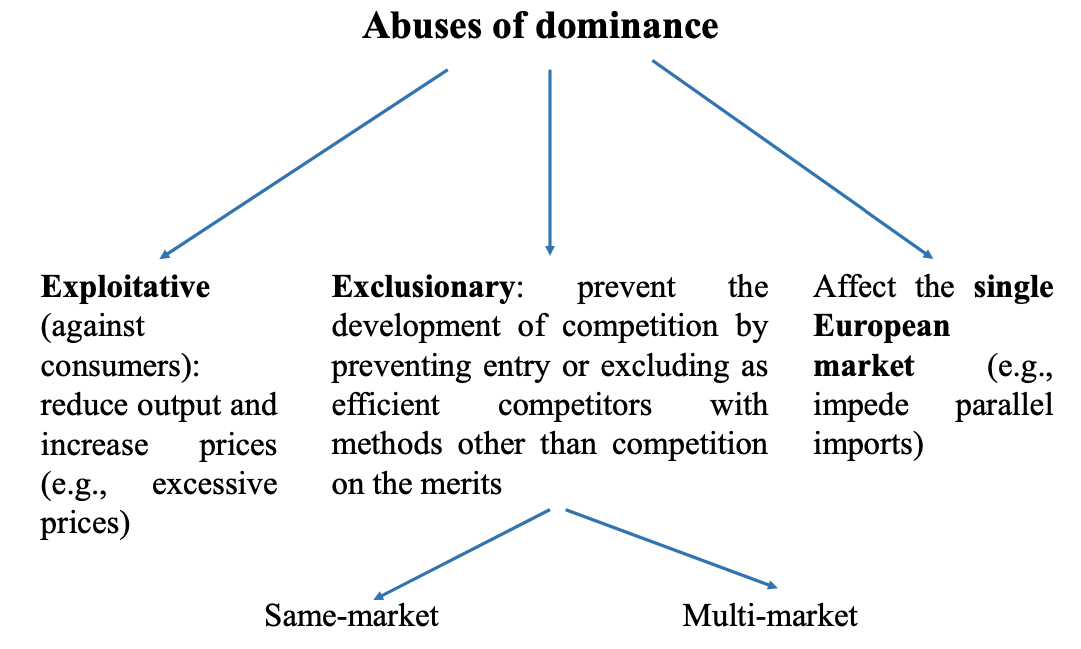
\includegraphics[width=0.6\linewidth]{types of abuses.png}
            \caption{Types of abuse}
        \end{figure}
    \end{center}

